\chapter{Introduction}

As stated in \cite{scilabstats2001}, Scilab's core provides
a complete set of features related to simulation and statistical
computations.
Indeed, Scilab provides uniform pseudo-random number generators, functions to 
compute the moments of a distribution and a complete set of 
distributions. In this document, we will make a complete 
overview on these features.

It must be noticed, though, that these features
are not as complete as in other languages, like R for example.
This is why several toolboxes have developped in order to extend 
the features of Scilab. In this document, we will present two
major toolboxes, that is the Sci\_R toolbox and the Stix toolbox.

In the last chapter, we will analyse the missing statistical 
features and will analyse how these features are available in other
tools, such as Matlab, R, or Octave.

\section{A sample session}

A good introduction on the statistical features of Scilab is \cite{scilabintro2007}.
In the remaining of this introduction chapter, we will try to have 
a flavour of how to perform statistical computations with Scilab.
We focus on the algorithms which are used inside Scilab, to show what 
exact algorithms perform the computations.

As a first example, we will generate a sequence of numbers from a 
normal law with mean 0 and standard deviation 1 (example inspired and simplified 
from \cite{scilabintro2007}). The probability density function (pdf) 
and the cumulated probability density function of the normal law is 
\begin{eqnarray}
f(x) &=& \frac{1}{\sqrt{2\pi}} e^{-\frac{t^2}{2}},\\
P(x) &=& \frac{1}{\sqrt{2\pi}} \int_{-\infty}^x e^{-\frac{t^2}{2}}.
\end{eqnarray}

The empirical cumulated density function \cite{artcomputerKnuthVol2} of a given
set of data $\{x_i\}_{i=1,N}$ is given by 
\begin{eqnarray}
F_N(x) &=& \frac{\textrm{number of } x_1,x_2,\ldots,x_n \textrm{ that are }\leq x}{N}.
\end{eqnarray}


The numerical method used by Scilab to generate such numbers is the Polar 
method for normal deviates, as presented in \cite{artcomputerKnuthVol2}.

\lstset{language=Scilab}
\lstset{numbers=left}
\lstset{basicstyle=\footnotesize}
\lstset{keywordstyle=\color{green}\bfseries}
\begin{lstlisting}
N=200;
x = rand(1,N,"normal");
Xsorted =gsort(x,"g","i"); 
Ydata = (1:N)/N;
plot(Xsorted,Ydata);
e=gce();
e.children.polyline_style=2;
xtitle("Empirical Cumulated Density Function of Normal Law with 200 samples")
filename = "introduction_ecdfnormal.png";
xs2png(0,filename);
\end{lstlisting}

The empirical cumulated density function 
is presented in figure \ref{introduction_ecdfnormal}.

\begin{figure}[htbp]
\begin{center}
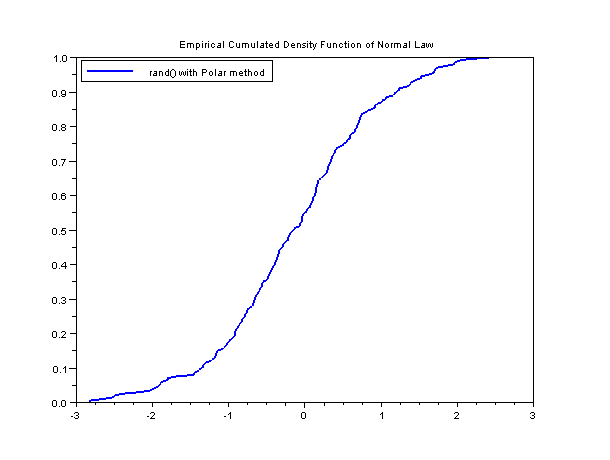
\includegraphics[height=10cm]{introduction_ecdfnormal.png}
\end{center}
\caption{Empirical Cumulated Density Function of Normal Law with 200 samples}
\label{introduction_ecdfnormal}
\end{figure}

To compare the data which is produced by rand with the 
cumulated density function of the normal law, we use the 
\emph{cdfnor} primitive. This primitive is based on \cite{Algorithm715}
and uses rational functions that theoretically approximate the normal 
distribution function to at least 18 significant decimal digits. The same 
primitive can be used to compute the inverse of the cumulated density 
function. In that case, rational functions are used as starting values to 
Newton's Iterations which compute the inverse standard normal.

\lstset{language=Scilab}
\lstset{numbers=left}
\lstset{basicstyle=\footnotesize}
\lstset{keywordstyle=\color{green}\bfseries}
\begin{lstlisting}
N=200;
x = rand(1,N,"normal");
Xsorted =gsort(x,"g","i"); 
Ydata = (1:N)/N;
x=linspace(-3,3,100);
P=cdfnor("PQ",x,zeros(x),ones(x));
plot(Xsorted,Ydata,x,P);
\end{lstlisting}

The comparison plot between the empirical cdf and the 
computed cdf is presented in figure \ref{introduction_ecdcomparison}.

\begin{figure}[htbp]
\begin{center}
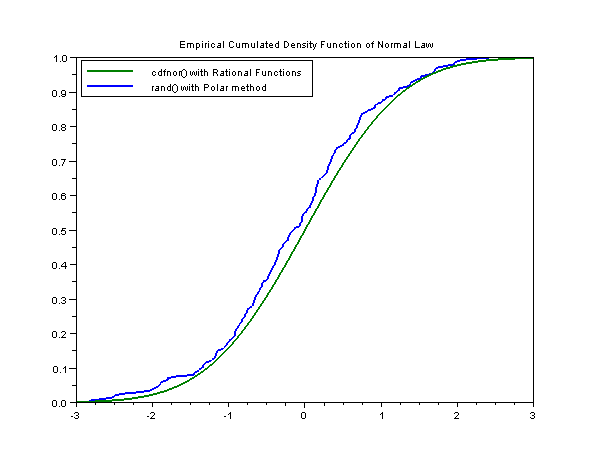
\includegraphics[height=10cm]{introduction_ecdfcomparison.png}
\end{center}
\caption{Cumulated Density Function of Normal Law : comparison of cdf from 
rational functions and empirical cdf from Polar method }
\label{introduction_ecdcomparison}
\end{figure}

The moments of a distribution can be computed with the 
\emph{mean}, \emph{variance} and \emph{stdev} Scilab macros,
which are implementations of the moments. For the variance
and standard deviation, the scaling factor is $N-1$.
In the following script, one computes these moment for 
an increasing number of samples, from $10^1$ to $10^5$.

\lstset{language=Scilab}
\lstset{numbers=left}
\lstset{basicstyle=\footnotesize}
\lstset{keywordstyle=\color{green}\bfseries}
\begin{lstlisting}
nbpoints = 5;
means=zeros(nbpoints,1);
vars=zeros(nbpoints,1);
stdevs=zeros(nbpoints,1);
nlist = 1:nbpoints;
for i = nlist
  N=10^i;
  x = rand(1,N,"normal");
  means(i) = mean(x);
  vars(i) = variance(x);
  stdevs(i) = stdev(x);
end
plot(nlist,[means,vars,stdevs]);
\end{lstlisting}

The convergence plot of the moments is presented in 
figure \ref{introduction_convergencemoments}.

\begin{figure}[htbp]
\begin{center}
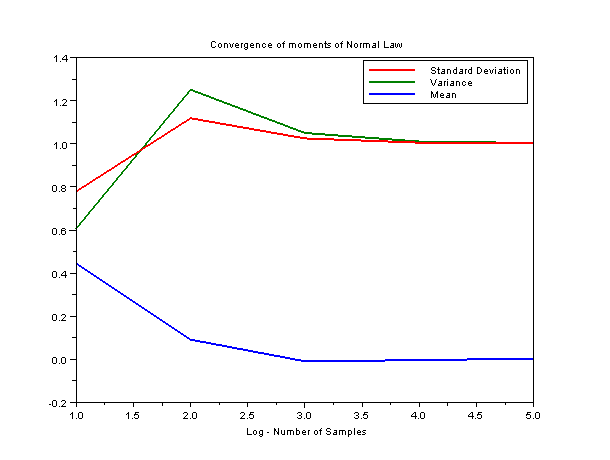
\includegraphics[height=10cm]{introduction_convergencemoments.png}
\end{center}
\caption{Convergence of the moments of the normal law}
\label{introduction_convergencemoments}
\end{figure}


